\documentclass[11pt]{article}

\usepackage{graphicx}
\usepackage{amsfonts}
\usepackage{amsmath}
\usepackage{amsthm}
\usepackage{latexsym}
\usepackage{amssymb}
\usepackage{hyperref}

\newtheorem{theorem}{Theorem}[section]
\newtheorem{lemma}[theorem]{Lemma}
\newtheorem{corollary}[theorem]{Corollary}
\newtheorem{assumption}[theorem]{Assumption}
\newtheorem{proposition}[theorem]{Proposition}
\newtheorem{observation}[theorem]{Observation}
\newtheorem{define}[theorem]{Definition}
\newtheorem{definition}[theorem]{Definition}
\newtheorem{example}[theorem]{Example}
\newtheorem{conjecture}[theorem]{Conjecture}
\newtheorem{claim}{Claim}

\pagestyle{plain}
\bibliographystyle{plain}

\title{K-Means Clustering}

\begin{document}

\maketitle

\section{Introduction}
\subsection{Clustering}
Unsupervised learning is a task that is used in machine learning. The data in unsupervised learning is not labeled. So, to find some meaningful information from this type of unlabeled data 
Clustering Algorithms have been evolved. Clustering is done on the data samples to find out the hidden patterns or some kind of information which cannot be predicted directly by looking into
those unlabeled data samples.Clustering divides the data into different groups based on the similarities and then label the data. Each group is called a cluster. Hence,``Clustering is a process of partitioning a set of data in to meaningful similar subclasses called clusters.''\\

We can show this with a simple graphical example: 

\begin{figure}
\begin{center}
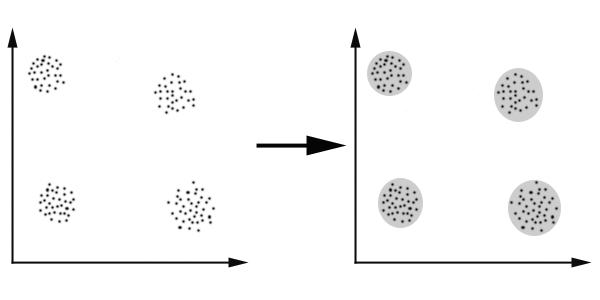
\includegraphics[scale=0.6]{clustering.jpg}
\end{center}
\end{figure}
\cite{fig_1}

\subsection{What is good clustering}
In order to get good quality clusters, better clustering methods should be implemented which should have high Intra-class similarities ( All the data points in that cluster should be similar to each others) \\
and should have Low-inter class similarity ( all the clusters should be dissimilar to each other)\\
To check if the clustering method is appropriate, the algorithm must satisfy all the following characteristics:\\


\subsubsection{Characteristics of Good Clustering Algorithm}
A good Clustering algorithm should satisfy the following requirements.\\
1. Scalability: The algorithm must be able to handle large number of data sets. That is, it should be able to cluster the entire data samples but not just a part of it.\\
2. It should have the ability to deal with all kinds of attributes. Example : Numerical, Binary.\\
3. It should be able to deal with noisy data and outliers ( data point which is far away from the clusters )\\
4. The algorithm should be able to find some or all the hidden patterns.\\
5. Dimensionality: The algorithm should be able to deal with the data samples that are high dimensional.\\ 

\section{Clustering Methods}

\subsection{Partitioning Method}
Clustering is based on data partitions,which means it helps to discover the groupings in the data by optimizing a specific objective function and iteratively improving the quality of partitions. \textbf{K-means} is an example for this type of clustering.\\
\subsection{Hierarchical Method}
This method is used to find new clusters using previously found ones. There are two kinds of hierarchical based algorithms.\\
For Agglomerative figure \cite{fig_2}
\subsubsection{Agglomerative method}
This method uses \textbf{Bottom- up-approach}.
If a set of points are considered in a Euclidean space. Each data point is initially  in a cluster of its own.at each step by finding the two closest clusters, the two clusters are merged into a single cluster.\\
The key operation of Hierarchy agglomerative clustering is to repeatedly combine the two nearest clusters in to a larger cluster.\\
The process stops when all groups are merged to one or k number of clusters is formed.



\begin{figure}\begin{center}
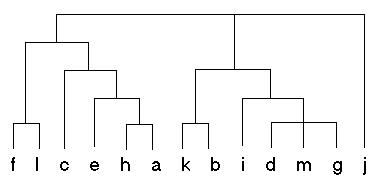
\includegraphics[scale=0.5]{Hierarch.jpg}
\end{center}
\end{figure}




\subsubsection{Divisive method}
This method uses \textbf{Top-down approach}.\\
The divisive method is opposite to Agglomerative method. In this all the data points belong single cluster to begin with and the cluster is recursively split into small clusters,\\
The iteration stops when the 'K' number or the desired number of clusters is formed.\\
\subsection{Density based method
}\\
Clustering is based on density which means the regions with sufficiently high density points are grouped under one cluster.\\
This kind of grouping helps in discovering the clusters of arbitrary shapes.\\
\subsection{Model based method}\\
For this type of clustering, model hypothesis is done for each cluster and tries to find the best fit of that model to each other.\\
\subsection{Graph based method}
  It deals only with the graphical data. There are nodes and node to node connections in the graph. Nodes are nothing but objects in this case and the clustering is done based on the connectivity of the nodes from one node to another node. This type of clustering is done in such a way that the nodes(objects) in the particular cluster are densely connected to one another and are very poorly connected with the nodes that belong to other clusters.\\
  

\section{Applications}\\

\subsection{Image Compression:}\\ K-means algorithm is used in image compression. k-means is used to sample every pixel of the image and the image can be represented using new limited number colors.

\subsection{Voice Biometrics:}\\ K-means helps in identify the voice sample data based on the gender of the speaker,voice modulation, pitch , emotion , accent etc.

\subsection{Marketing:}\\ Marketing uses clustering technique to cluster the customer with high salary and target on them i.e., when a manager in bank wants to offer loans to their customers. They will collect the information of their customers with high salary and concentrate on them.

\subsection{Libraries:}\\ Grouping similar books or books of same subjects at a place in order to identify them easily.

\subsection{WWW:}\\ In world wide web Clustering helps to identify all the documents related to the topic which was searched.
\\

\section{K-Means Clustering}\\
\subsection{History}
The term "k-means" was first used by James MacQueen in 1967, though the idea goes back to Hugo Steinhaus in 1957. The standard algorithm was first proposed by Stuart Lloyd in 1957 
as a technique for pulse-code modulation, though it wasn't published outside of Bell Labs until 1982. In 1965, E. W. Forgy published essentially the same method, which is why it is
sometimes referred to as Lloyd-Forgy. \cite{wiki_his}
\\

\subsection{K-Means} 
K-means is one of the best known clustering algorithm to solve the unsupervised learning issue. Assume a data set with ‘n’ data points $ x_i $ , i=1...n that have to be partitioned 
into k clusters and the goal is to assign each data point to the nearest cluster. The aim of the algorithm is to find the positions "$ \mu_i $" , i=1...k of the clusters that minimize the 
distance from the data points to the cluster centers $ \mu_i $ . Here,$ \mu_i $ i=1...k  are the centroids of the K clusters which are fixed a priority.\\
\\
Initialize a centroid (center) point for one for each cluster that is denoted by $ \mu $. These centers should be chosen randomly in such a way that the each center is possibly far away from each other. Because the number of clusters and the cluster position might alter the final solution.\\
\\
After determining the centroids for each cluster, all the data points should be assigned to the centroid in such a way the distance between the centroid and data point is minimum.\\
\\
That means each point is assigned to the closest centroid and that collection of the points that are assigned to the centroid forms a cluster. The centroids are updated based on the data points that belong to the cluster. Then all the data points are again assigned to the newly updated centroids and thus it changes the initial cluster positions. After forming the new clusters the centroids are again updated. The assigning and updating the centroids are repeated until no data point changes in the cluster or the centroid position remains the same.\\
\\
For figure refer \cite{fig_3}\\
This algorithm aims at minimizing an objective function known as squared error function given by:\\  

\\
\sum_{i=1}^{k} \sum_{j=1}^{ki}(\mid\mid $x_i$-$ \mu_j $\mid\mid})^{2} = J(V)
\\

{\mid\mid $ x_i $ - $\mu_j $\mid\mid} \textbf{is the Euclidean distance between $ x_i $ and $ \mu_i $}\\

‘$ k_i $ is the number of \textbf{data points in $ i^th $ cluster}\\

‘k’ is the number of \textbf{cluster centers}.\\


The Step by step iteration of the k-means algorithm is shown in the above diagram:\\



\begin{figure}\begin{center}
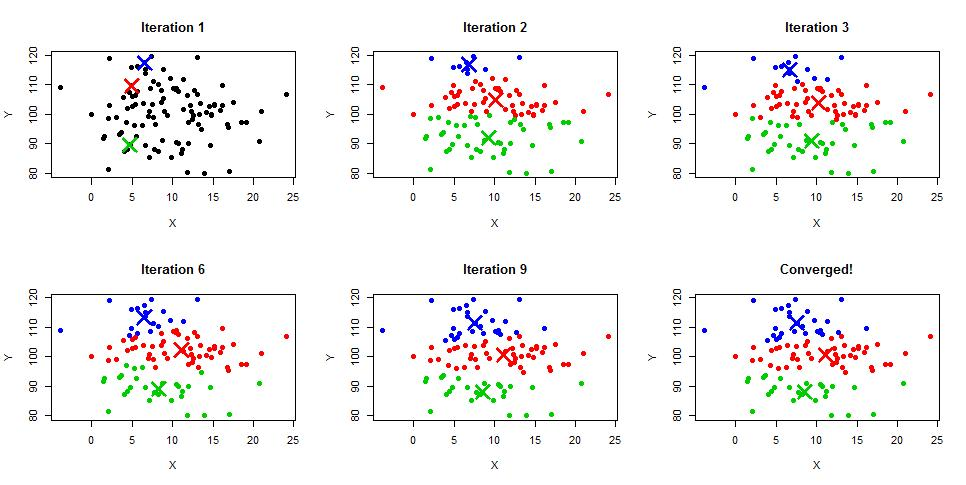
\includegraphics[scale=0.5]{sk1.jpg}
\end{center}

\end{figure}


	In the above example, there are n data points. Three random centroids are chosen from the n data points i.e., k= 3. Then the nearest data points are assigned to each centroid thus forming a new cluster shown in iteration.\\

	The centroids are then updated based on the data points in the cluster. The assignment of data points to the newly updated centroids is shown in iteration.\\
	
	This process is repeated until convergence. That means this process is repeated until the data points in the clusters are constant or the updated centroid position is constant. The last iteration shows the final cluster output. 

\subsection{ALGORITHM:}

Step 1: Initialize 'k' number of clusters and the cluster centroids $ \mu_1 $,$ \mu_2 $, $ \mu_3 $ .... $ \mu_k $ randomly for $ x_i $,i=1..n data points.\\
Step 2: Repeat\\
Step 3: Assign each data point to $ \mu_i $ ,i =1...k such that the distance between the data points is minimum among the k clusters.\\
Step 4: Re-calculate the mean for each cluster based on the data points assigned to the each cluster.\\

\textbf{COMPUTING MEAN}\\

\mu = \dfrac{1}{ki} \sum_{i=1}^{ ki } $x_i$ \\


where, $ k_i $ represents number of data points in $ i^th $ cluster.\\

Step 5: Repeat the algorithm until no change.\\

\subsection{ASSIGNING POINTS TO THE CLOSEST CENTROID:}\\
To assign points to the closest centroid in the k-means algorithm often the Euclidean Distance measure is used for the data points in Euclidean space.\\
There are many other proximity measures other than Euclidean distance. Manhattan Distance can also be applied to measure the distance for the Euclidean Data. \\

\subsection{MEAN COMPUTATION AND OBJECTIVE FUNCTION:}\\
Mean Computation is nothing but calculating the centroid for each cluster. The data points that belong to the cluster might alter at every step. So, the mean value changes at every single iteration.\\
Example: Consider three data points (x1,y1),(x2,y2),(x3,y3) which are two dimensional that belongs to one cluster.\\

Then the mean μ for the cluster is,\\
$\mu$ = \dfrac{x1+x2+x3}{3} ,\dfrac{y1+y2+y3}{3}\\

Using the above formula the mean is calculated in every step of the k-means clustering algorithm.\\


\subsection{OBJECTIVE FUNCTION OR THE SQUARED ERROR FUNCTION:}\\

The objective function measures the quality of the clustering. The aim of the algorithm is to minimize the squared error function or the Objective function. For the squared error function the error of each data point i.e., its Euclidean distance from its nearest centroid is calculated and then total sum of the squared errors is computed. When there are two different sets of clusters that are produced by two different runs of K-means, the one with smallest squared error distance is preferred because the centroids for those clusters with minimum squared error distance have better representation of the points in their particular clusters.


\subsection{Code Implimentation:}

Our Project has two different parts\\
1.To generate the points\\
2.K-Means operation\\
\\
First we run "DrawPoint.java" and after selecting the points 
we execute "kmeans.java" and give the desired dimensions and number of centroids.
\\
Generation of points is done using DrawPoints.java and Area.java.
DrawPoints.java is executable and uses ``buildDynamicPointAddition'' method to get the popup screen.
"redrawCursor" is used to get the x and y cordintaes of the cursor.
"updateClickPoint" is used to update the selected points in the destination file.\\
\\
For K-Means we use "kmeans.java" and "DataPoint.java"\\
As every Program Execution starts at main, the program takes file name as input and stores it in ``file-name''. 
Later it takes the number of dimensions to work on and stores it in ``nod'' and asks for centroids to store it in ``noc''. These are the inputs needed.\\
\\
Later the execution starts with reading file line by line, reads the values based on ``nod'' and stores into DataPoint object.
``setfacet'' method is used to store all values into dataPoint.
Facets variable based on ``noc'', number of centroids are assigned in order. 
After completion of reading the file, required fields in files based on nod and centroids are made.\\
\\
Next assigning of centroids: ``AssignCentroids'' method is used to assign centroids. Here euclidean distance is calculated using
``getEuclideanDistance'' method. By the euclidean distance, calculate the centroid with lowest distance assigned to each point, 
based on assigned centroid, cluster is assigned here by ``setCluster'' method\\
\\
Updating centroids: Here the Centroid is updated by calculating mean, for this ``updateCentroids'' method is been used.
Here again the assigning of centroids will takes place. This process takes place untill the error is less than 0.001.
The error is calculated while updating the centroids. mean while in this process we increment cycles variable to know how
many times the process is executed to get the desired output.\\
\\

\subsection{Advantages of k-means clustering}\\

K-means algorithm has many advantages compared to that of other clustering algorithms like \textbf{hierarchy} and \textbf{fuzzy-c} algorithm.
	1. Efficiency : K- means algorithm is relatively efficient because of its low time complexity O(tkn), where n is objects, k is number of clusters and t is the number of iterations.\\
	2. It is very easy to implement and simple to understand.\\
	
\section{K-means ++}\\

\subsection{K-Means ++ (careful seeding)} is an advancement of k-means algorithm where the centroids are chosen carefully. The need to specify the k clusters in advance is a major drawback in the k-means algorithm. The output depends on the initial number of clusters declared.\\
	So, the output changes for the different input cluster numbers which may not give the desired clusters and the data may be interpreted incorrectly.
K-means algorithm is also not suitable to discover the clusters with non-convex shape. To overcome these disadvantages \textbf{K-means ++} came into use.\\

\subsection{Working of K-means ++ :}
 \\
Step 1: Only the initial centroid is determined at uniformly random.\\
Step 2: The remaining centroids are determined based on the probability proportional to the distance measure from the initial centroid. Thus avoiding the formation of overlapped and unwanted number of clusters.\\
Step 3: Same procedure as the standard k-means algorithm.\\

\bibliography{latex}

\end{document}
